
\chapter{Getting started with PETSc}
\label{chap:getstarted}

\section{A code that does almost nothing, but in parallel}

The purpose of the \PETSc library is to help you solve scientific and engineering problems, such as PDEs, on multi-processor computers.  As \PETSc is built ``on top of'' the Message Passing Interface (MPI; \citep{Groppetal1999}) library, some of the MPI flavor comes through.  Therefore we start with an an introductory MPI code which calls \PETSc for some basic tasks.

This code \texttt{c1e.c}, shown in its entirety in Figure \ref{code:e}, approximates Euler's constant
\begin{equation}
e = \sum_{n = 0}^\infty \frac{1}{n!} \approx 2.718281828 \label{introeseries}
\end{equation}
It does the computation in a distributed manner by computing one term of the infinite series on each process.  Thus it computes a better estimate of $e$ when run on more MPI processes. While this is a silly use of \PETSc, it is an easy-to-understand parallel computation.

As with any C source code, \texttt{c1e.c} has a function called \texttt{main()} which takes inputs from the command line, namely \texttt{argc} and \texttt{argv},\sidenote{Here \texttt{argc} is an \texttt{int} holding the argument count and \texttt{argv} is an array of strings (i.e.~type \texttt{char**}) holding the command line including all arguments.  However, in all codes in this book we simply pass these arguments on to \PETSc through the \texttt{PetscInitialize()} method.  \PETSc extracts options through this mechanism.} and which outputs an \texttt{int}.  The output is $0$ if the program succeeds.  Also like all C codes, we include needed headers.  Only \texttt{petsc.h} is needed.

The substance of \texttt{c1e.c} is to declare some variables, do a computation on each process, and communicate the results between processes to get an estimate of $e$.

Before we can compile and run \texttt{c1e.c}, \PETSc must be installed.  If it is not already available, go to
\begin{quote}
\href{http://www.mcs.anl.gov/petsc/download/index.html}{\texttt{www.mcs.anl.gov/petsc/download/}}
\end{quote}
to download the source code, and then follow the instructions at
\begin{quote}
\href{http://www.mcs.anl.gov/petsc/documentation/installation.html}{\texttt{www.mcs.anl.gov/petsc/documentation/installation.html}}
\end{quote}
to install.  Be sure to run ``\texttt{make test}'' and see it pass the tests.  If \PETSc is correctly installed then  environment variables \texttt{PETSC\_DIR} and \texttt{PETSC\_ARCH} point to a valid installation, and the MPI command \texttt{mpiexec} is from the same MPI installation as was used in configuring \PETSc.\sidenote{Type ``\texttt{which mpiexec}'' to find which one you are running.  You may need to modify your \texttt{PATH} environment variable to get the right \texttt{mpiexec}.}

Do the following to compile \texttt{c1e.c}:
\begin{cline}
$ cd p4pdes/c/
$ make c1e
\end{cline}
%$
Calling ``\texttt{make}'' uses \texttt{p4pdes/c/makefile}.  An extract of this makefile is shown in Figure \ref{code:c1emakefile}.  For all the codes in this book, the makefile has this form, as recommended in the \PETSc \emph{User's Manual} \citep{petsc-user-ref}.

\inputwhole{../c/ch1/e.c}{\texttt{p4pdes/c/ch1/e.c}}{Compute $e$ in parallel with \PETSc.}{code:e}

Run the code like this:
\begin{cline}
$ ./c1e
e is about 1.000000000000000
rank 0 did 1 flops
\end{cline}
%$
The value $1.0$ is a very poor estimate of $e$, but this code does better with more MPI processes:
\begin{cline}
$ mpiexec -n 5 ./c1e
e is about 2.708333333333333
rank 0 did 0 flops
rank 4 did 3 flops
rank 2 did 1 flops
rank 3 did 2 flops
rank 1 did 0 flops
\end{cline}
%$
That's a better estimate of $e$, but hardly impressive.  On the other hand, with $N=20$ processes, and thus $N=20$ terms in series \eqref{introeseries}, we get a good estimate:
\begin{cline}
$ mpiexec -n 20 ./c1e
e is about 2.718281828459045
rank 0 did 0 flops
...
\end{cline}
%$

\cinputraw{ch1makefile.frag}{extract from \texttt{p4pdes/ch1/makefile}}{All \texttt{makefile}s for our \PETSc codes look like this.}{}{//START}{//STOP}{code:ch1makefile}

Perhaps the reader is now worried that this book was written using a large supercomputer whereas the reader has a little laptop with only a couple of cores.  In fact these five or twenty process runs work just fine on the author's laptop.  MPI processes are created as needed, using an old feature of operating systems: multitasking.  Speedup from parallelism is another matter; we will return to it.

The main job in \texttt{c1e.c} is to collect the sum of the terms of series \eqref{introeseries} onto each process.  Each process computes term $1/n!$, where $n$ is returned by \texttt{MPI\_Comm\_rank()}.  More precisely, \texttt{PETSC\_COMM\_WORLD} is an MPI communicator \citep{Groppetal1999} containing all processes generated by \texttt{mpiexec} in the above calls, and $n$ is the rank of the process in this communicator.  Then a call to \texttt{MPI\_Allreduce()} does the sum and then sends it back to each process.  These direct uses of the MPI library are a part of using \PETSc because \PETSc generally avoids duplicating MPI functionality.

We print the computed estimate of $e$, but each process also prints its rank and the work it did.  The formatted print command \texttt{PetscPrintf()}, which is like \texttt{fprintf()} from the C standard library, is called twice, once with MPI communicator \texttt{PETSC\_COMM\_WORLD} and once with \texttt{PETSC\_COMM\_SELF}.  The first of these printing jobs is \emph{collective} over all processes, and thus only done once, while the second is individual to each rank.\sidenote{A process is often just called a \emph{rank} in MPI language.}  In the output the \texttt{PETSC\_COMM\_SELF} printed lines can appear in random order because the print occurs as soon as that process reaches that line.

Every \PETSc program should start and end with the commands \texttt{PetscInitialize()} and \texttt{PetscFinalize()}:
\begin{code}
PetscInitialize(&argc,&args,(char*)0,help);
... everything else goes here ...
PetscFinalize();
\end{code}
As an argument to \texttt{PetscInitialize()} we supply a \texttt{help} string.  This string is a good place to say what is the purpose of the code.  To see the help string, and a longer list of possible \PETSc options, do:
\begin{cline}
$ ./c1e -help
\end{cline}
%$
or
\begin{cline}
$ ./c1e -help | less
\end{cline}
%$
Through \texttt{-help}, \PETSc programs have a built-in help system for runtime options that is both light-weight and surprisingly-effective.  For example, to see options related to logging performance, do
\begin{cline}
$ ./c1e -help | grep log_
\end{cline}
%$
We will see later how to add options to our own programs so that they will be documented in the same way.

Unfortunately, \texttt{c1e.c} and all other \PETSc programs have error-checking clutter.  While languages other than C might help with decluttering, we are stuck with ugly lines that look like
\begin{code}
ierr = PetscCommand(...); CHKERRQ(ierr);
\end{code}
The explanation is that almost all \PETSc methods, and most user-written methods in \PETSc programs, return an \texttt{int} for error checking, with value $0$ if successful.  In the line above, \texttt{ierr} is passed to the \texttt{CHKERRQ()} macro which does nothing if \texttt{ierr == 0} but which stops the program with a ``traceback'' otherwise.\sidenote{A traceback is a list of the nested methods, in reverse order, showing the line numbers and method names of the location where the error occurred.}  This traceback mechanism tends to be the first line of defense when debugging run-time errors.  It is most effective if \PETSc is configured with debugging symbols, i.e.~with the option \texttt{--with-debugging=1}.

Examples in this book always capture-and-check the returned error code using \texttt{ierr} and \texttt{CHKERRQ()}; these are always present in the \texttt{.c} sources in \texttt{p4pde/c/}.  However, after this chapter we will strip the ``\texttt{ierr =}'' and ``\texttt{CHKERRQ(ierr);}'' clutter from the code displayed in the text.


\section{Linear systems}

Our goal is to compute more interesting quantities than Euler's constant $e$.  At the core of most \PETSc computations is a finite-dimensional linear system.  Before solving such systems in \PETSc, we recall the most basic ideas of numerical linear algebra.

Suppose $\bb\in \RR^{N}$ is a column vector and $A\in\RR^{N\times N}$ is a square matrix.  The linear system
\begin{equation}
A \bu = \bb \label{introsystem}
\end{equation}
has a unique solution if $A$ is invertible, namely
\begin{equation}
\bu = A^{-1} \bb. \label{introsolution}
\end{equation}
This is simple in theory.

It is not so simple in practice, however, to solve large systems on a computer.  There are two key facts to keep in mind while working numerically  \citep{TrefethenBau}:
\renewcommand{\labelenumi}{\roman{enumi})}
\begin{enumerate}
\item \label{limittoaccuracy} \emph{limit to accuracy}:  If real numbers are represented on the computer with machine precision $\eps$ then the solution of \eqref{introsystem} can only be computed within an error $\kappa(A) \eps$ where $\kappa(A) = \|A\|_2 \|A^{-1}\|_2$ is the (2-norm) \emph{condition number} of $A$.
\item \emph{cost of direct solutions}:  Computation of solution \eqref{introsolution} by a direct method like Gauss elimination,\sidenote{Or by QR, so that we have a \emph{backward stable} direct method.} whether actually forming $A^{-1}$ or not, is an $O(N^3)$ operation.
\end{enumerate}

Fact i) is about \emph{conditioning} not \emph{methods}.  Informally speaking, there are linear systems that are the same to within $\eps$ but for which the infinite-precision solutions $\bu$ differ by an amount $\kappa(A) \eps$.

On modern computers the precision for the C \texttt{double} type, the default 64-bit representation of real numbers, is $\eps = 2.2 \times 10^{-16}$.  Thus by i), a linear system having $\kappa(A) \approx 10^{10}$, for example, can only be solved to about six digits of precision.  While a matrix with such a large condition number is ``poorly-conditioned,'' it is easy to reach that level for $\kappa(A)$ when discretizing PDEs.  We have to be aware of conditioning when forming expectations about solution accuracy.

By ii) a generic linear system with $N=10^6$ equations requires $10^{18}$ or so operations to solve by Gauss elimination.  Even modern supercomputers take a while to do a quintillion operations.  However, though Gauss elimination is impractical for systems of $N=10^6$ equations, we will successfully solve PDE-generated linear systems of this size on a single processor in a few seconds, and in $O(N)$ operations, in Chapter \ref{chap:multigrid}.  The key fact that discretized PDEs generate linear systems with exploitable structure, especially \emph{sparsity} but also coefficient smoothness, will have to be exposed in serious numerical PDE solutions because naive application of direct methods is too slow.
%time ./c4poisson -da_refine 7 -ksp_type cg -pc_type mg
%on 1153 x 1153 grid:  iterations 2, residual norm = 1.88082e-05
%real 11.18


\section{\PETSc \pVec and \pMat objects}

To build our first \PETSc code to solve a linear system, we need the \emph{objects} which hold vectors (\pVec) and matrices (\pMat).  Note that, although \PETSc is written in C, and not C++ for example, it is a relentlessly object-oriented software library.  Consider the operations which create and configure a matrix object \texttt{A} for linear system \eqref{introsystem}:
\begin{code}
Mat A;
MatCreate(COMM,&A);
MatSetSizes(A,PETSC_DECIDE,PETSC_DECIDE,N,N);
MatSetOptionsPrefix(A,"a_");
MatSetFromOptions(A);
... fill entries of (i.e. assemble) A ...
... solve system with A ...
MatDestroy(&A);
\end{code}
We can think of these calls as using methods ``owned'' by the \pMat type, in the sense that they manipulate the internal representation of a \pMat, which is, happily, hidden from us.  If not true ``objects'', major \PETSc types are at least abstract data types with a hidden implementation.

The act of filling entries will treat a \PETSc \pMat as an abstract object.  In fact, a \pMat need not even have entries because it might, instead, contain code that applies a linear operator to vectors.  Furthermore the data structure inside a \pMat depends on runtime choices, the most basic being that the number of bytes used to store entries on a given MPI process will depend on the number of processes.

For all \PETSc object types this basic sequence of operations applies:\sidenote{Here ``\texttt{Object}'' is a meta-name for a \PETSc type like \pVec or \pMat.}
\begin{code}
Object X;
ObjectCreate(COMM,&X);
... code sets properties of X ...
ObjectSetFromOptions(X);  // allows run-time setting
                          // or overriding of properties
... code uses X ...
ObjectDestroy(&X);
\end{code}

Because \PETSc objects are generally distributed across, and accessible from, multiple MPI processes, the first argument of an \texttt{ObjectCreate()} method is an MPI communicator (``\texttt{COMM}'').  We will usually use \texttt{PETSC\_COMM\_WORLD} as it is the default communicator formed from all \texttt{N} processes when we start a run with ``\texttt{mpiexec -n N}.''  All processes in \texttt{COMM} must call the \texttt{ObjectCreate()} and  \texttt{ObjectDestroy()} methods.  That is, these are ``collective'' operations.

In the \pMat code above, note the call to \texttt{MatSetOptionsPrefix()}.  Through this ``prefix'', run-time options can address the particular \pMat object.  For example, the run-time option \texttt{-a\_mat\_view} will print out the entries of \texttt{A}.  An option prefix like ``\texttt{a\_}'' is especially helpful in distinguishing multiple \pMat objects at the command line.

Once \pMat \texttt{A} is created and set up by the first several commands \texttt{MatCreate()}--\texttt{MatSetFromOptions()}, then various methods become valid for \texttt{A}, for example including the \texttt{MatSetValues()} method to set entries in \texttt{A}.  We will use that method after looking at the parallel layout of vectors and matrices.


\section{Assembly and parallel layout of \pVecs and \pMats}

A \pVec or \pMat stores its entries in parallel across all the processes in the MPI communicator used when creating it.  For example, the create-assemble sequence of a \pVec with four entries might look like
\begin{code}
Vec x;
PetscInt   i[4] = {0, 1, 2, 3};
PetscReal  v[4] = {11.0, 7.0, 5.0, 3.0};

VecCreate(COMM,&x);
VecSetSizes(x,PETSC_DECIDE,4);
VecSetFromOptions(x);
VecSetValues(x,4,i,v,INSERT_VALUES);
VecAssemblyBegin(x);
VecAssemblyEnd(x);
\end{code}
The four entries of \texttt{Vec x} are set by \texttt{VecSetValues()}, putting values from array \texttt{v} at the indices given by \texttt{i}.

The operation of setting values in \texttt{x} may require communication between processes because entries which are to be stored on one process could be set by another process.  Such communication occurs between the \texttt{VecAssemblyBegin()} and \texttt{VecAssemblyEnd()} commands.

\begin{marginfigure}
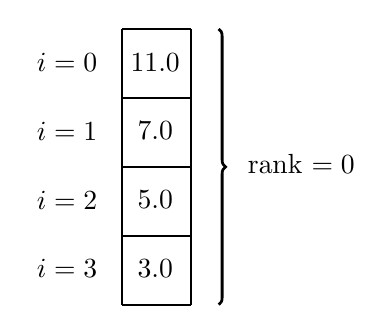
\begin{tikzpicture}[scale=3.5]
  \pgfmathsetmacro\fourth{1.0/4.0}
  \pgfmathsetmacro\xoff{0.12}
  \pgfmathsetmacro\yoff{0.12}
  \draw[xstep=\fourth,ystep=\fourth,black,thick] (0.0,0.0) grid (\fourth,1.0);
  \node at (-0.2,1.0-\yoff) {$i=0$};
  \node at (\xoff,1.0-\yoff) {$11.0$};
  \node at (-0.2,0.75-\yoff) {$i=1$};
  \node at (\xoff,0.75-\yoff) {$7.0$};
  \node at (-0.2,0.5-\yoff) {$i=2$};
  \node at (\xoff,0.5-\yoff) {$5.0$};
  \node at (-0.2,0.25-\yoff) {$i=3$};
  \node at (\xoff,0.25-\yoff) {$3.0$};
  \draw[decoration={brace,mirror,raise=5pt},decorate,line width=1pt] (0.3,0.0) -- (0.3,1.0);
  \node at (0.65,0.51) {rank $=0$};
\end{tikzpicture}
\bigskip
\caption{A sequential \pVec layout, all on rank $=0$ process.}
\label{fig:seqveclayout}
\end{marginfigure}

The reader is allowed to think of a \PETSc \pVec as a one-dimensional C array with its contents split across the processes in the MPI communicator used in the \texttt{VecCreate()} command.  For example, if the above code appears in \texttt{mycode.c}, and if it is run sequentially on one process, i.e.~as
\begin{cline}
$ ./mycode.c
\end{cline}
%$
then, at the end of the above create-set-assemble sequence, the storage of \texttt{x} looks like Figure \ref{fig:seqveclayout}.  However, if run as
\begin{cline}
$ mpiexec -n 2 ./mycode.c
\end{cline}
%$
then the layout looks like Figure \ref{fig:mpitwoveclayout}.  In this case the argument \texttt{PETSC\_DECIDE} in \texttt{VecSetSizes()} is active, and the decision is to put the first two entries of \texttt{x} on the rank $0$ process and the other two on the rank $1$ process. 

\begin{marginfigure}
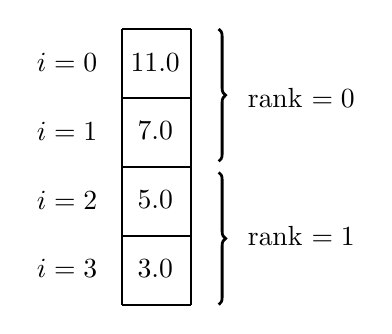
\begin{tikzpicture}[scale=3.5]
  \pgfmathsetmacro\fourth{1.0/4.0}
  \pgfmathsetmacro\xoff{0.12}
  \pgfmathsetmacro\yoff{0.12}
  \draw[xstep=\fourth,ystep=\fourth,black,thick] (0.0,0.0) grid (\fourth,1.0);
  \node at (-0.2,1.0-\yoff) {$i=0$};
  \node at (\xoff,1.0-\yoff) {$11.0$};
  \node at (-0.2,0.75-\yoff) {$i=1$};
  \node at (\xoff,0.75-\yoff) {$7.0$};
  \node at (-0.2,0.5-\yoff) {$i=2$};
  \node at (\xoff,0.5-\yoff) {$5.0$};
  \node at (-0.2,0.25-\yoff) {$i=3$};
  \node at (\xoff,0.25-\yoff) {$3.0$};
  \draw[decoration={brace,mirror,raise=5pt},decorate,line width=1pt] (0.3,0.52) -- (0.3,1.0);
  \node at (0.65,0.752) {rank $=0$};
  \draw[decoration={brace,mirror,raise=5pt},decorate,line width=1pt] (0.3,0.0) -- (0.3,0.48);
  \node at (0.65,0.251) {rank $=1$};
\end{tikzpicture}
\bigskip
\caption{A parallel \pVec layout on two processes.  Because we call ``\texttt{VecSetSizes(x,PETSC\_DECIDE,4)}'', \PETSc decides to split the storage in the middle.}
\label{fig:mpitwoveclayout}
\end{marginfigure}

\pMat objects, however, are not actually 2D C arrays even in serial (i.e.~in one-process runs).  Compared to \pVecs they require additional choices regarding parallel distribution.  Though this is hidden inside the implementation of \pMat, the most common storage format is \emph{parallel compressed sparse row storage}, what \PETSc calls the \texttt{MATMPIAIJ} type.  In this type a range of rows is owned by each process (parallel row storage), and within each owned range of rows only the specifically-allocated\sidenote{These are generally the nonzero entries, and usually referred-to as such.} entries are stored (sparse), and furthermore nonzero entries are stored contiguously in memory along with an additional index array (compressed).

\pMat objects are linear operators so their major purpose is to multiply \pVecs.  The result vector of a \pMat-\pVec product is a linear combination of the columns of the \pMat.  Thus, in practice, ``parallel row storage'' of the \pMat means these things:
\begin{itemize}
\item \PETSc internally distributes the rows of the \pMat $A$ the same way as the entries of the intended \emph{output} (i.e.~column) \pVec.  Thus if $Ax=b$ for some $x$ then row $i$ of $A$ is on the rank $m$ processor if and if entry $i$ of $b$ is on the rank $m$ processor.  (At least this can be expected when \texttt{PETSC\_DECIDE} is used in setting both the \pVec and \pMat sizes and they are of the same dimension.)
\item Before \PETSc computes a \pMat-\pVec product, \PETSc communicates (``scatters'') the whole \pVec to each process.
\item After the scatter the \pMat-\pVec product is a local operation, requiring no further communication.
\end{itemize}

But one doesn't really need to know all this to assemble a \pMat!  For example, here is how to create and assemble a $4\times 4$ \pMat one row at a time:
\begin{code}
Mat A;
PetscInt  i, j[4] = {0, 1, 2, 3};
PetscReal v[4];

MatCreate(PETSC_COMM_WORLD,&A);
MatSetSizes(A,PETSC_DECIDE,PETSC_DECIDE,4,4);
MatSetFromOptions(A);
MatSetUp(A);

i = 0;  v[0] = 1.0;  v[1] = 2.0;  v[2] = 3.0;
MatSetValues(A,1,&i,3,j,v,INSERT_VALUES);
i = 1;  v[0] = 2.0;  v[1] = 1.0;  v[2] = -2.0;  v[3] = -3.0;
MatSetValues(A,1,&i,4,j,v,INSERT_VALUES);
i = 2;  v[0] = -1.0;  v[1] = 1.0;  v[2] = 1.0;  v[3] = 0.0;
MatSetValues(A,1,&i,4,j,v,INSERT_VALUES);
j[0] = 1;  j[1] = 2;  j[2] = 3;
i = 3;  v[0] = 1.0;  v[1] = 1.0;  v[2] = -1.0;
MatSetValues(A,1,&i,3,j,v,INSERT_VALUES);

MatAssemblyBegin(A,MAT_FINAL_ASSEMBLY);
MatAssemblyEnd(A,MAT_FINAL_ASSEMBLY);
\end{code}
The method \texttt{MatSetValues()} sets multiple values, in this case a row.  The ``\texttt{1,\&i}'' arguments to \texttt{MatSetValues()} say that we are setting one row with global index \texttt{i}.  The ``\texttt{3,j}'' or ``\texttt{4,j}'' arguments say that we set the row using integer array \texttt{j} for the (global) column indices.

\begin{marginfigure}
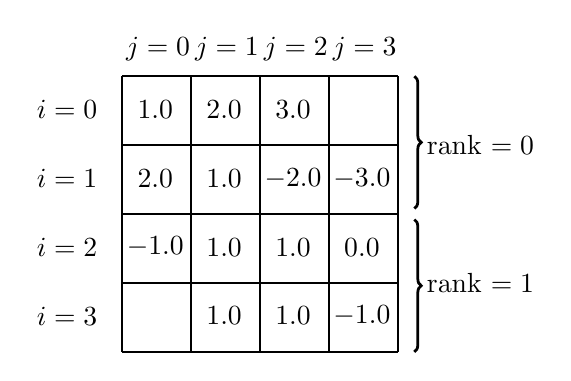
\begin{tikzpicture}[scale=3.5]
  \pgfmathsetmacro\fourth{1.0/4.0}
  \pgfmathsetmacro\xoff{0.12}
  \pgfmathsetmacro\yoff{0.12}
  \draw[xstep=\fourth,ystep=\fourth,black,thick] (0.0,0.0) grid (1.0,1.0);

  \node at (-0.2, 1.0-\yoff) {$i=0$};
  \node at (-0.2,0.75-\yoff) {$i=1$};
  \node at (-0.2, 0.5-\yoff) {$i=2$};
  \node at (-0.2,0.25-\yoff) {$i=3$};

  \node at ( 1.0-\xoff, 1.1) {$j=3$};
  \node at (0.75-\xoff, 1.1) {$j=2$};
  \node at ( 0.5-\xoff, 1.1) {$j=1$};
  \node at (0.25-\xoff, 1.1) {$j=0$};

  \node at (\xoff,1.0-\yoff) {$1.0$};
  \node at (0.25+\xoff,1.0-\yoff) {$2.0$};
  \node at (0.5+\xoff,1.0-\yoff) {$3.0$};
  \node at (0.75+\xoff,1.0-\yoff) {};

  \node at (\xoff,0.75-\yoff) {$2.0$};
  \node at (0.25+\xoff,0.75-\yoff) {$1.0$};
  \node at (0.5+\xoff,0.75-\yoff) {$-2.0$};
  \node at (0.75+\xoff,0.75-\yoff) {$-3.0$};

  \node at (\xoff,0.5-\yoff) {$-1.0$};
  \node at (0.25+\xoff,0.5-\yoff) {$1.0$};
  \node at (0.5+\xoff,0.5-\yoff) {$1.0$};
  \node at (0.75+\xoff,0.5-\yoff) {$0.0$};

  \node at (\xoff,0.25-\yoff) {};
  \node at (0.25+\xoff,0.25-\yoff) {$1.0$};
  \node at (0.5+\xoff,0.25-\yoff) {$1.0$};
  \node at (0.75+\xoff,0.25-\yoff) {$-1.0$};

  \draw[decoration={brace,mirror,raise=5pt},decorate,line width=1pt] (1.01,0.52) -- (1.01,1.0);
  \node at (1.3,0.752) {rank $=0$};
  \draw[decoration={brace,mirror,raise=5pt},decorate,line width=1pt] (1.01,0.0) -- (1.01,0.48);
  \node at (1.3,0.251) {rank $=1$};
\end{tikzpicture}
\bigskip
\caption{A parallel \pMat layout on two processes.  Blank entries are not allocated.}
\label{fig:mpitwomatlayout}
\end{marginfigure}

If the above lines appeared in \texttt{mycode.c}, and if it was run
\begin{cline}
$ mpiexec -n 2 ./mycode
\end{cline}
%$
then the layout would be as in Figure \ref{fig:mpitwomatlayout}.

We can have \PETSc show us the entries in the \pMat in different formats at the command line:
\begin{cline}
$ ./mycode -mat_view
Mat Object: 1 MPI processes
  type: seqaij
row 0: (0, 1)  (1, 2)  (2, 3)
row 1: (0, 2)  (1, 1)  (2, -2)  (3, -3)
row 2: (0, -1)  (1, 1)  (2, 1)  (3, 0)
row 3: (1, 1)  (2, 1)  (3, -1)
$ ./mycode -mat_view ::ascii_dense
Mat Object: 1 MPI processes
  type: seqaij
 1.00000e+00  2.00000e+00  3.00000e+00  0.00000e+00
 2.00000e+00  1.00000e+00  -2.00000e+00  -3.00000e+00
 -1.00000e+00  1.00000e+00  1.00000e+00  0.00000e+00
 0.00000e+00  1.00000e+00  1.00000e+00  -1.00000e+00
\end{cline}
The first view shows the compressed sparse storage, with values as pairs with column index and value.  The second view is a traditional (``dense'') display where all zero values are shown, whether allocated or not.\sidenote{Other possibilities, not shown, are \texttt{-mat\_view ::ascii\_matlab}, which dumps in Matlab's text format, and \texttt{-mat\_view binary -viewer\_binary\_filename a.dat} which saves to file \texttt{a.dat} in \PETSc's scalable binary format.}  Note that \texttt{-mat\_view} output is activated by the \texttt{MatAssemblyBegin/End()} calls.

In these cases the matrix was stored in \emph{serial} compressed sparse row format, the \texttt{MATSEQAIJ} type, because of the one-process execution.  If the code is run in parallel, i.e.~by \texttt{mpiexec -n N ./mycode}, then \texttt{-mat\_view}  reports \texttt{type:~mpiaij} corresponding to \pMat type \texttt{MATMPIAIJ}.  This is the ``parallel compressed sparse row storage'' described above.


\section{Numerical linear algebra: residual, iteration, preconditioning}

Direct methods like Gauss elimination \citep{TrefethenBau} are one way to solve a linear system.  The most powerful methods for our later PDE-solving uses, however, are iterative.  They use the \emph{residual} of some approximation of the solution to the linear system.

By definition, the residual of $\bu_0$ in linear system \eqref{introsystem} is the vector
\begin{equation}
\br_0 = \bb - A \bu_0. \label{residualdefn}
\end{equation}
Evaluating the residual for a known vector $\bu_0$ requires only applying $A$ to it, an $O(N^2)$ operation at worst.  Because most discretization schemes for PDEs generate matrices $A$ that are \emph{sparse}, with many more zero entries than nonzeros, and because often the number of nonzeros per row is small and independent of $N$, the operation $A\bu_0$ and the evaluation of the residual can usually be done in $O(N)$ operations.

The \emph{Richardson iteration}, which simply adds a multiple $\omega$ of the last residual at each step,
\begin{equation}
\bu_{k+1} = \bu_k + \omega (\bb - A \bu_k),  \label{introrichardson}
\end{equation}
is an example of an iterative method based on the residual.  If significantly fewer than $O(N^2)$ steps are needed to make $\bu_k$ an adequate approximation of the exact solution $\bu$, then the Richardson iteration can improve on Gauss elimination.  On the other hand, the Richardson iteration may not converge, as in the next Example.

\newcommand{\rvect}[3]{\ensuremath{\bu_{#1} = \begin{bmatrix} #2 \\ #3 \end{bmatrix}}}

\medskip\noindent\hrulefill
\begin{example} Consider the linear system
\begin{equation}
A \bu
= \begin{bmatrix}
10 & -1 \\ -1 & 1
\end{bmatrix}
\begin{bmatrix} u_1 \\ u_2 \end{bmatrix}
= \begin{bmatrix} 8 \\ 1 \end{bmatrix}
= \bb
 \label{introexample}
\end{equation}
which has solution $\bu = [1\,\, 2]^\top$.  If we start with estimate $\bu_0 = [0\,\, 0]^\top$ then the $\omega=1$ Richardson iteration \eqref{introrichardson} gives a sequence of vectors % see ../matlab/richardsonex.m
\begin{equation}
\rvect{0}{0}{0}, \rvect{1}{8}{1}, \rvect{2}{-63}{9}, \rvect{3}{584}{-62}, \dots
\end{equation}
This sequence is not heading toward the solution.
\end{example}
\noindent\hrulefill

\medskip
If we rewrite \eqref{introrichardson} as
\begin{equation}
\bu_{k+1} = (I - \omega A) \bu_k + \omega \bb  \label{introrewriterichardson}
\end{equation}
then it is easy to believe that the ``size'' of the matrix $I-\omega A$ will determine whether $\lim_{k\to\infty} \bu_k$ exists.

To make this precise we recall important definitions.  A complex number $\lambda \in \CC$ is an \emph{eigenvalue} of a square matrix $B\in\RR^{N\times N}$ if there is a nonzero vector $\bv\in\CC^N$ so that $B \bv = \lambda \bv$.  The set of all eigenvalues of $B$ is the \emph{spectrum} $\sigma(B)$ of $B$.  The \emph{singular values} are the square roots of the eigenvalues of the matrix $B^*B$, a symmetric and positive-definite matrix with nonnegative eigenvalues.  Singular values are geometrically-defined as the lengths of semi-axes of the ellipsoid in $\RR^N$ that results from applying $B$ to all vectors in the unit ball of $\RR^N$ \citep{TrefethenBau}.

Properties of matrices described in terms of eigenvalues or singular values are generically called ``spectral properties.''  For example, because $\|B\|_2$ is equal to the largest singular value of $B$, while $\|B^{-1}\|_2$ is equal to the inverse of the smallest singular value of $B$, these are spectral properties.  The 2-norm condition number $\kappa(B)=\|B\|_2/\|B^{-1}\|_2$ is thus a spectral property as well; it is visualized as the eccentricity of the ellipsoid above.

It is an easy exercise to show that the Richardson iteration \eqref{introrichardson} will converge if and only if all the eigenvalues of $B=I-\omega A$ are inside the unit circle.  Defining the \emph{spectral radius} $\rho(B)$ as the maximum magnitude of the eigenvalues of $B$, we can describe the convergence of the Richardson iteration:
\begin{equation}
\text{\eqref{introrichardson} converges if and only if } \rho(I-\omega A) < 1. \label{introconvergethm}
\end{equation}
One can also show that $\rho(B) \le \|B\|_2$, so \eqref{introrewriterichardson} converges if $\|I-\omega A\|_2 < 1$.

Considering spectral properties brings us to the important general point that there are many other systems which are equivalent to \eqref{introsystem}.  In fact, if $P\in\RR^{N\times N}$ is an invertible square matrix then the systems
\begin{equation}
(P^{-1} A) \bu = P^{-1} \bb \label{introleftpre}
\end{equation}
and
\begin{equation}
(A P^{-1}) (P\bu) = \bb \label{introrightpre}
\end{equation}
have the same solution(s) $\bu$ as \eqref{introsystem}.  However, matrices $P^{-1} A$ or $A P^{-1}$ generally have different eigenvalues, condition numbers, and so on---different spectral properties---from $A$.  While the accuracy of the approximate solution $\bu$ cannot be improved beyond the $\kappa(A) \eps$ level, as fact i) on page \pageref{limittoaccuracy} cannot be overcome, methods can take advantage of better spectral properties to generate $\bu$ more quickly.  This idea is effective if $P^{-1}$ is easy to apply, in the sense of low computational cost.

Equivalent systems \eqref{introleftpre} and \eqref{introrightpre} are referred to as \emph{preconditioned} systems, with \eqref{introleftpre} called \emph{left preconditioning} and \eqref{introrightpre} called \emph{right-preconditioning}.  The next example shows how preconditioning can make the Richardson iteration converge.

\medskip\noindent\hrulefill
\begin{examplecont}  Suppose we use the diagonal matrix from  \eqref{introexample} as $P$:
\begin{equation}
P = \begin{bmatrix}
10 & 0 \\ 0 & 1
\end{bmatrix}.  \label{introP}
\end{equation}
Being diagonal, this $P$ is easy to invert and apply.  The preconditioned Richardson iteration using $P$, namely
\begin{equation}
\bu_{k+1} = \bu_k + \omega (P^{-1} \bb - P^{-1} A \bu_k),  \label{introprerichardson}
\end{equation}
is better behaved.  With $\bu_0 = [0\,\, 0]^*$ again we get this sequence from \eqref{introprerichardson}:
\begin{equation}
\rvect{0}{0}{0}, \rvect{1}{0.8}{1.0}, \rvect{2}{0.9}{1.8}, \rvect{3}{0.98}{1.90}, \dots
\end{equation}
This sequence is apparently going to $\bu = [1\,\, 2]^*$.  The explanation is not hard to see; compare
\begin{equation}
\rho(I-A) = -9.1, \qquad \rho(I-P^{-1} A) = 0.32.
\end{equation}
This example illustrates convergence claim \eqref{introconvergethm}.
\end{examplecont}
\noindent\hrulefill

\medskip
Preconditioning using the diagonal as in the above example is called \emph{Jacobi} preconditioning.  It is related to, but not the same idea as, the classical Jacobi iteration \citep{Greenbaum1997} for solving a linear system.


\section{Numerical linear algebra: Krylov space methods}

The most powerful iterative methods for solving system \eqref{introsystem} generate optimal, in various senses \citep{TrefethenBau}, estimates $\bu_k$ which are linear combinations of vectors $\bz,A\bz,A^2\bz,\dots,A^{k-1}\bz$ where $\bz$ is a fixed vector (which is often $\bz=\bb$).  These methods are collectively called \emph{Krylov space methods} because the span of such vectors is a \emph{Krylov space}.  Examples of such methods include the Richardson iteration, conjugate gradients (CG), and minimum residual methods (e.g.~MINRES or GMRES; \citet{Greenbaum1997,Saad2003}).  The classical Jacobi and Gauss-Siedel \citep{Greenbaum1997} iterative methods are not Krylov space methods because they involve extracting parts of (entries of) $A$ as a matrix.  The effectiveness of a given Krylov method on a system depends on the eigenvalues or singular values of the matrix $A$, i.e.~on its spectral properties.  As many Krylov space methods are built into and fully-supported by \PETSc, we will use them heavily in all later Chapters.

To be concrete, given $\bb$ the $n$th Krylov space in defined to be
    $$\mathcal{K}_n = \operatorname{span}\{\bb,A\bb,A^2\bb,\dots,A^{n-1}\bb\}.$$
Suppose $\tilde\bu \in \mathcal{K}_n$ so
    $$\tilde\bu = c_0 \bb + c_1 A \bb + c_2 A^2 \bb + \dots + c_{n-1} A^{n-1} \bb,$$
or equivalently
    $$\tilde\bu = p_{n-1}(A) \bb$$
for the $n-1$ degree polynomial $p_{n-1}(x) = c_0 + c_1 x + \dots + c_{n-1} x^{n-1}$ applied to $A$.  Thus if we want $\tilde\bu$ to approximate $\bu$, the solution to \eqref{introsystem}, then we want to find a polynomial $p_{n-1}$ so that
    $$p_{n-1}(A) \approx A^{-1}.$$
Krylov space methods do this, subject to the important idea that if $p_{n-1}(z)$ is close to $1/z$ \emph{on the finite set of eigenvalues of} $A$, i.e.~on the spectrum $\sigma(A)\subset \CC$, then $p_{n-1}(A) \approx A^{-1}$.  Thus, whether $p_{n-1}$ is a ``good'' polynomial for approximately inverting $A$ is a spectral question about $A$.

For example, consider the Richardson iteration \eqref{introrichardson}, namely $\bu_{k+1} = \bu_k + \omega (\bb - A \bu_k)$

FIXME

\begin{figure}
\bigskip
\includegraphics[width=0.9\textwidth]{richpolyplot}
\caption{(FIXME: improve caption and move to Chapter 1)  The Richardson iteration \eqref{introrichardson} is equivalent to approximating $\bu=A^{-1}\bb$ by using these polynomials $p_k(x)$ to approximate $p_k(A)\approx A^{-1}$.}
\label{fig:richpolyplot}
\end{figure}

FIXME: flesh out CG and GMRES

Most Krylov methods are implemented in \PETSc, and we get access to them via a \pKSP object.  Which method is used can be controlled at runtime, and runtime experimentation is always appropriate.  For the Poisson problem in Chapter \ref{chap:structured}, for example, we will see that preconditioned CG is very effective, but eventually we will put the most emphasis on the preconditioning stage and see that multigrid is extraordinarily effective for that purpose (see Chapter \ref{chap:multigrid}).  We will return to Krylov space methods repeatedly in later Chapters.

Our brief introduction of iterative linear algebra is hardly adequate.  But we need now to return to \PETSc codes and solve linear systems.  In the upcoming material the reader can first treat \PETSc's linear solver object as a black box, but then explore how it works through runtime options.

\vfill
\clearpage
\newpage
\section{Solve a small linear system in \PETSc}

We already know how to create, fill, and destroy \pVec and \pMat objects.  The next code, \texttt{c1vecmatksp.c} shown in Figure \ref{code:vecmatksp}, does these steps.  To actually solve a linear system it also uses a Krylov space method object ``\pKSP''.  This linear solver uses a method chosen at runtime.

Besides the expected \texttt{Create/SetFromOptions/Destroy} sequence for \pKSP, there are two important commands needed even for the simplest examples.  First we need to tell \pKSP about the matrix in the linear system by the command
\begin{code}
KSPSetOperators(ksp,A,A);
\end{code}
Then the system is actually solved by
\begin{code}
KSPSolve(ksp,b,x);
\end{code}
which also supplies the right-hand side of the system (i.e.~an allocated and assembled \pVec \texttt{b}) and space for the solution (i.e.~an allocated \pVec \texttt{x}).

Why do we list \texttt{A} twice in calling \texttt{KSPSetOperators()}?  Recall the linear system $A\bx=\bb$ is equivalent to $P^{-1} A \bx = P^{-1} \bb$ (left preconditioning).  At runtime we are going to choose a preconditioning method which builds $P^{-1}$ from $A$ or from an approximation of $A$.  For example, \emph{incomplete LU} factorization of $A$ can be used in generating $P^{-1}$, or $P$ could be the diagonal of $A$ (as in the example above).  The second matrix argument to \texttt{KSPSetOperators()} is the \pMat from which $P^{-1}$ is built.  Note we do not supply $P$ itself, as that would require the user to write extra code.  It would also block easy choice among preconditioners at runtime.  Instead we supply ``material'' from which the preconditioner is built, and the most common such material is $A$ itself.

After calling \texttt{KSPSolve()} we display the solution \pVec by calling \texttt{VecView()}.  This and everything else about the code in Figure \ref{code:vecmatksp} should now be self-explanatory.  So let's run it:
\begin{cline}
$ make c1vecmatksp
$ ./c1vecmatksp
Vec Object: 1 MPI processes
  type: seq
1
0
2
-1
\end{cline}
This solves the system and gives us $\bx$.  But what happened and how to control it?

\inputwhole{../c/ch2/vecmatksp.c}{\texttt{p4pdes/c/c1vecmatksp.c}}{Solve a small linear system.}{code:vecmatksp}


\section{Revealing solvers at runtime}

To start to see what happened when we ran \texttt{./c1vecmatksp} above, we could start by viewing the \pVec and \pMat objects.  The result of ``\texttt{./c1vecmatksp -vec\_view -mat\_view}'' is perfectly clear, but it tells us nothing about the solver, and it gives no hints on alternative ways of solving the equations.

Here is a key idea which cannot be over-emphasized:
\begin{quote}
\emph{learning \PETSc requires viewing \emph{solver} objects at runtime.}
\end{quote}
Here we try \texttt{-ksp\_view}; the output is slightly-clipped for clarity:
\begin{cline}
$ ./c1vecmatksp -ksp_view
KSP Object: 1 MPI processes
  type: gmres
    GMRES: restart=30, using Classical (unmodified) Gram-Schmidt ...
    GMRES: happy breakdown tolerance 1e-30
  maximum iterations=10000, initial guess is zero
  tolerances:  relative=1e-05, absolute=1e-50, divergence=10000
  left preconditioning
  using PRECONDITIONED norm type for convergence test
PC Object: 1 MPI processes
  type: ilu
    ILU: out-of-place factorization
    0 levels of fill
    tolerance for zero pivot 2.22045e-14
    matrix ordering: natural
    factor fill ratio given 1, needed 1
      ...
  linear system matrix = precond matrix:
  Mat Object:   1 MPI processes
    type: seqaij
    rows=4, cols=4
    total: nonzeros=16, allocated nonzeros=20
    total number of mallocs used during MatSetValues calls =0
      using I-node routines: found 1 nodes, limit used is 5
Vec Object: 1 MPI processes
  type: seq
1
0
2
-1
\end{cline}
%$
Here is some of what we learn:
\begin{itemize}
\item The default \pKSP solver is GMRES \citep{Saad2003}.\sidenote{This is \texttt{-ksp\_type gmres} as a command-line option.}
\item As GMRES builds an approximation of the solution from the Krylov space by saving more and more vectors, and thus uses up memory, one restarts after a number of iterations.  The default is \texttt{-ksp\_gmres\_restart 30}.
\item The default convergence tolerances for the \pKSP are \texttt{-ksp\_rtol 1.0e-5} and \texttt{-ksp\_atol 1.0e-50}.  In particular, \pKSP iterations stop when the residual norm has been reduced by $10^5$.
\item Inside the \pKSP is a \pPC preconditioner object.  We did not have to ask for one in the code, as every \pKSP has a \pPC.
\item The default \pPC is left preconditioning with ILU, i.e.~incomplete LU factorization, which is \texttt{-pc\_type ilu} as a runtime option.\sidenote{We will see in a moment that this is the \emph{serial} default \pPC, and there is more going on in parallel.}
\item Actually, the preconditioner is usually called ``ILU($0$)'', i.e.~with ``\texttt{0 levels of fill}'', so it does not use more memory than used by $A$ already.
\item The \pPC object has a copy of $A$ (``\texttt{Mat Object}''), because it was supplied as the second argument to \texttt{KSPSetOperators()} above.
\end{itemize}
Of course, we get the solution $\bx$ too.

While option \texttt{-ksp\_view} tells us what the solver \emph{is}, option \texttt{-ksp\_monitor} shows what it \emph{does}.  In this case, the \pKSP iteration is short:
\begin{cline}
$ ./c1vecmatksp -ksp_monitor
  0 KSP Residual norm 2.449489742783e+00
  1 KSP Residual norm 1.520235486122e-15
Vec Object: 1 MPI processes
...
\end{cline}
%$
The reason that the residual drops to nearly zero in one iteration is that GMRES sees a preconditioned system with an identity matrix in this case.  That is, $P^{-1} A = I$ because the ILU operation on this particular $A$ is actually a full LU factorization.  Our $A$ is banded and ``dense enough'' so that the LU factorization requires no fill-in.

For a small system like this a direct solve also works fine.  To see how to do it, first do
\begin{cline}
$ ./c1vecmatksp -help | grep ksp_type
  -ksp_type <gmres>: Krylov method (one of) cg ... preonly ... (KSPSetType)
$ ./c1vecmatksp -help | grep pc_type
  -pc_type <ilu>: Preconditioner (one of) none jacobi ... lu ... (PCSetType)
\end{cline}
to see the many solver and preconditioner options.  One of the preconditioners is ``\texttt{lu}'', suggesting a direct solve.  In this case we \emph{do not} want iterations, and one of the \pKSP options is ``\texttt{preonly}''.  Thus the direct solver combination we want is
\begin{cline}
$ ./c1vecmatksp -ksp_type preonly -pc_type lu
\end{cline}
%$
The reader should check that the output of \texttt{-ksp\_view} is as intended.\sidenote{The output of \texttt{-ksp\_monitor} is empty as there were, in fact, no iterations!}

When solving on multiple processors, using ILU($0$) as the default preconditioner makes no sense.  This is because, even when fill-in is avoided, the LU factorization algorithm would involve a great deal of interprocessor communication.  However, there are blocks along the diagonal of the system matrix $A$ which are entirely owned by a single processor.  The ILU($0$) method can be applied to these, and the result treated as an approximation $P^{-1}\approx A^{-1}$.  That is, the blocks along the diagonal can be approximately inverted by ILU($0$), and the result treated as a diagonal (i.e.~Jacobi) preconditioner.  So this is what is done by default \PETSc \pKSP settings in parallel:
\begin{itemize}
\item The default \pKSP is still GMRES with restart 30.
\item The default \pPC is \texttt{bjacobi}, i.e.~application of approximate diagonal-block inverses as $P^{-1}$.
\item Inside the \pPC is a \texttt{sub\_pc} object, also a \pPC, which is ILU($0$).\sidenote{There is even a \texttt{sub\_ksp} object, but it is \texttt{preonly}.  So let's just ignore that complication for now.}
\item These defaults correspond to options
\begin{quote}
\texttt{-ksp\_type gmres -pc\_type bjacobi -sub\_pc\_type ilu}
\end{quote}
\end{itemize}
The reader can confirm this understanding of the situation by running
\begin{cline}
mpiexec -n 2 ./c1vecmatksp -ksp_view
\end{cline}
But surely that's enough runtime options for now.  There will be more, especially in later chapters when we solve PDEs.

\section{More \PETSc functionality from the code side}

We have seen \PETSc code to set up and solve linear systems, but there is more to say.  The next example \texttt{c1tri.c}, split into Figures \ref{code:tripartone} and \ref{code:triparttwo}, introduces these additional concepts and their associated function calls:
\begin{enumerate}
\item Creating an option, so that the size of the linear system can be controlled at runtime, by using \texttt{PetscOptionsXXX()} calls.
\item Using \texttt{VecDuplicate()} for allocation.
\item Assembling a system of arbitrary size across an arbitrary number of processes, using \texttt{MatGetOwnershipRange()} to only set locally-owned rows.
\item Using \texttt{VecAXPY()}, \texttt{VecNorm()}, and \texttt{PetscPrintf()} to compute and display the error in a case where the exact solution is known.
\end{enumerate}

\vfill
\newpage
\cinputpartnostrip{ch2/tri.c}{Set up \pVec and \pMat objects for a tridiagonal system.}{I}{//STARTSETUP}{//ENDSETUP}{code:tripartone}

First build (``\texttt{make c1tri}'') and run the code with options that show what it is does by default:
\begin{cline}
$ ./c1tri -ksp_monitor -a_mat_view ::ascii_dense
Mat Object:(a_) 1 MPI processes
  type: seqaij
  3.00000e+00  -1.00000e+00   0.00000e+00   0.00000e+00 
 -1.00000e+00   3.00000e+00  -1.00000e+00   0.00000e+00 
  0.00000e+00  -1.00000e+00   3.00000e+00  -1.00000e+00 
  0.00000e+00   0.00000e+00  -1.00000e+00   3.00000e+00 
  0 KSP Residual norm 3.302822756884e+00 
  1 KSP Residual norm 5.519370044893e-16 
error for m = 4 system is |x-xexact|_2 = 5.1e-16
\end{cline}
%$

To get started on the new concepts shown in Figure \ref{code:tripartone}, notice that methods \texttt{PetscOptionsBegin()} and \texttt{PetscOptionsEnd()} bracket the call to \texttt{PetscOptionsInt()}.  We set an option prefix ``\texttt{-tri\_...}'' so that the new option we create is distinguished from the many built-in \PETSc options that start with \texttt{-ksp\_...} or \texttt{-vec\_...} or whatever.  Our use of \texttt{PetscOptionsInt()} creates an option \texttt{-tri\_m} which allows the user to set the variable \texttt{m}, and to leave the default \texttt{m}$=4$ unaltered if the option is not set.

To see the option and its default value in \texttt{-help} output do
\begin{cline}
$ make c1tri
$ ./c1tri -help | grep tri_
Solve a tridiagonal system of arbitrary size.  Option prefix = tri_.
  -tri_m <4>: dimension of linear system (None)
\end{cline}
Here, for instance, we reset the system size to be small and we view the matrix:
\begin{cline}
$ ./c1tri -tri_m 2 -a_mat_view
Mat Object:(a_) 1 MPI processes
  type: seqaij
row 0: (0, 3)  (1, -1) 
row 1: (0, -1)  (1, 3) 
error for m = 2 system is |x-xexact|_2 = 8.0e-16
\end{cline}
%$

After setting up the new option, next in \texttt{c1tri.c} the numerical solution \pVec \texttt{x} is created just as we did in the last example \texttt{c1vecmatksp.c} (Figure \ref{code:vecmatksp}).  But now we also want to create \pVecs \texttt{b} and \texttt{xexact}; the former is the right-hand side of the linear system and the latter holds the exact solution to the linear system so that we can evaluate the error in the numerical solution.  Though at this stage we have not filled any entries of \texttt{x}, we can save repetitive function calls to \texttt{VecCreate/SetSizes/SetFromOptions()} when creating these additional \pVecs.  That is, because they have the same properties and parallel layout we can use \texttt{VecDuplicate()} to allocate \pVecs just like \texttt{x}.\sidenote{There is a different method for copying the contents of \pVecs, namely \texttt{VecCopy()}.  It requires that the two \pVecs are already allocated and have the same layout.}

Next we assemble the matrix $A$.  This is a boring tridiagonal matrix with $3$ on the diagonal and $-1$ in the super- and sub-diagonals.  Though boring, we want to assemble it efficiently in parallel, something that will be important when solving 2D and 3D PDEs in later chapters.  However, only when \texttt{c1tri.c} is run do we know how many processes are in use.  A key method for efficient matrix assembly in parallel is the method \texttt{MatGetOwnershipRange()} which tells our program, as it is running on a particular process (rank), what rows it owns locally.  In the case of a many structured matrices like this one, we can avoid all interprocess communication by assembling exactly the rows we own.  As seen at the top of Figure \ref{code:triparttwo}, we call
\begin{quote}
\texttt{MatGetOwnershipRange(A,\&Istart,\&Iend)}
\end{quote}
to get the starting and ending row indices for the local process.  These are used as limits in a \texttt{for} loop over the locally own rows, wherein we call \texttt{MatSetValues()} to actually set the entries of $A$.  We call \texttt{MatAssemblyBegin/End()} to complete the assembly of $A$.

\cinputpartnostrip{ch2/tri.c}{Assemble and solve.}{II}{//ENDSETUP}{//ENDSOLVE}{code:triparttwo}

We need to assemble the right-hand side $\bb$ of the linear system.  But this is related to the question: how does one get the exact solution $\bx_{\text{exact}}$ to a linear system $A\bx_{\text{exact}} = \bb$?  The easiest way for demonstration purposes, as here, is to \emph{choose} $\bx_{\text{exact}}$ and then compute $\bb$ by multiplying by $A$.  Thus, we set (unimportant) values for \texttt{xexact}, and call \texttt{VecAssemblyBegin/End()} on it.  Then we compute \texttt{b} by calling \texttt{MatMult(A,xexact,b)}.

As in the earlier code, we set up  the \pKSP and then call \texttt{KSPSolve()} to approximately solve $A\bx = \bb$.  As the \pKSP is working we can see it reduce the $k$th-iteration residual norm $\|\bb-A\bx_k\|_2$ just by using option \texttt{-ksp\_monitor}.  In this case we also want to see that the actual error
	$$\|\bx - \bx_{\text{exact}}\|_2$$
is small when the \pKSP completes its work.  So, after getting \texttt{x} from \texttt{KSPSolve()} we compute the error with two commands,

\medskip
\begin{tabular}{lcrcl}
\text{\texttt{VecAXPY(x,-1.0,xexact)}}       & : & $\bx$                   & $\leftarrow$ & $-1\, \bx_{\text{exact}} + \bx$ \\
\text{\texttt{VecNorm(x,NORM\_2,\&errnorm)}} & : & \text{\texttt{errnorm}} & $\leftarrow$ & $\|\bx\|_2$.
\end{tabular}

\medskip
\noindent and then print \texttt{errnorm} by calling \texttt{PetscPrintf()}.


\section{A first look at performance}

The linear system assembled by \texttt{c1tri.c} is about as easy to solve as they get.   It is tridiagonal, symmetric, diagonally-dominant, and positive definite.\sidenote{Regarding the last property, see exercise \ref{exer:computeeigs}.}  So \PETSc ought to be able to solve it quickly, and parallelization ought to be effective.

\newcommand{\WORKSTATION}{\textsc{workstation}\xspace}
We can time a one-process solution:\sidenote{On the author's 2012-era workstation with 16 GB memory and a single Intel Core i7-3820 8-core cpu running at 3.60GHz.  We call this machine \WORKSTATION. \label{defineworkstation}}
\begin{cline}
$ time ./c1tri -tri_m 10000
error for m = 10000 system is |x-xexact|_2 = 8.0e-13
real 0.04
user 0.04
sys 0.00
\end{cline}
%$
Only the ``\texttt{real}'' time is worth considering, so from now on we will use an alias to get just this time:
\begin{cline}
$ alias timer='time -f "real %e"'
\end{cline}
%$

The above timing result of $.04$ seconds suggests that this $m=10^4$ dimension system is not yet big enough to be worth testing, so we experiment on what $m$ gives a linear system with noticeable solution time.  Here is a roll-your-own bash loop\sidenote{I have found \href{http://mywiki.wooledge.org/FullBashGuide}{mywiki.wooledge.org/ FullBashGuide} to be a reasonable online overview of bash.} to time some bigger solves:
\begin{cline}
$ for M in 10000 100000 1000000 10000000; do timer ./c1tri -tri_m $M; done
error for m = 10000 system is |x-xexact|_2 = 8.0e-13
real 0.04
error for m = 100000 system is |x-xexact|_2 = 3.1e-12
real 0.18
error for m = 1000000 system is |x-xexact|_2 = 4.8e-11
real 1.17
error for m = 10000000 system is |x-xexact|_2 = 3.5e-10
real 11.96
\end{cline}
Thus the default methods\sidenote{Recall: GMRES with ILU($0$) preconditioning.} solve a system of size $m=10^7$ (ten million) in a time of about 12 seconds.

It is reasonable to ask if other methods and/or more processors speed up the solution of the linear system of size $m=10^7$.  In particular we can try a direct solve (\texttt{-ksp\_type preonly -pc\_type lu}), the default serial solver (\texttt{-ksp\_type gmres -pc\_type ilu}), and the default parallel solver (\texttt{-ksp\_type gmres -pc\_type bjacobi -sub\_pc\_type ilu}).  We can turn off preconditioning (\texttt{-pc\_type none}) or switch from ILU($0$)-based preconditioning to Jacobi preconditioning (\texttt{-pc\_type jacobi}). 

To generate Table \ref{tab:c1tritiming} below, we did:
\begin{cline}
$ timer mpiexec -n N ./c1tri -tri_m 10000000 -ksp_rtol 1.0e-10 -ksp_type KSP -pc_type PC
\end{cline}
%$
for $N=1$ and $N=4$, and several \pKSP/\pPC choices.  The tighter tolerance \texttt{-ksp\_rtol 1.0e-10} was added because a fair comparison of iterative and direct methods needs significant accuracy in the iterative ones.

\newcommand{\intime}[1]{\input{../c/ch2/timing/tri/#1}}
\begin{figure}[ht]
\texttt{
\begin{tabular}{llll}
\underline{KSP}\hspace{0.5in} & \underline{PC}\hspace{0.8in} & \underline{N=1 \textrm{time (s)}}\hspace{0.3in} & \underline{N=4 \textrm{time (s)}} \\
preonly    & lu          & \intime{preonly.lu.1}       &  \\
           & cholesky    & \intime{preonly.cholesky.1} &  \\
richardson & jacobi      & \intime{richardson.jacobi.1}& \intime{richardson.jacobi.4} \\
gmres      & none        & \intime{gmres.none.1}       & \intime{gmres.none.4} \\
           & jacobi      & \intime{gmres.jacobi.1}     & \intime{gmres.jacobi.4} \\
           & ilu         & \intime{gmres.ilu.1}        &  \\
           & bjacobi/ilu &                             & \intime{gmres.bjacobi.4} \\
cg         & none        & \intime{cg.none.1}          & \intime{cg.none.4} \\
           & jacobi      & \intime{cg.jacobi.1}        & \intime{cg.jacobi.4} \\
           & icc         & \intime{cg.icc.1}           &  \\
           & bjacobi/icc &                             & \intime{cg.bjacobi.4} \\
\end{tabular}
}
\caption{Times for \texttt{c1tri.c} to solve systems of dimension $m=10^7$.  In this case the matrix is \emph{tridiagonal}, \emph{symmetric}, \emph{diagonally-dominant}, and \emph{positive definite}.  All runs were on \WORKSTATION (see page \pageref{defineworkstation}).} \label{tab:c1tritiming}
\end{figure}

This table deserves discussion:
\begin{itemize}
\item Entries ``\texttt{bjacobi/ilu}'' and ``\texttt{bjacobi/icc}'' correspond to options \texttt{-pc\_type bjacobi -sub\_pc\_type ilu} and \texttt{-pc\_type bjacobi -sub\_pc\_type icc}, respectively.  As already noted, the first of these is the parallel default.\sidenote{This table, at least, suggests it is a reasonable choice for that purpose.}
\item Counting floating point operations shows the leading-order work for Cholesky is $m^3/3$ while for LU it is $2 m^3/3$ \citep{TrefethenBau}.  This is reflected in the direct-solve results (with \texttt{-ksp\_type preonly}).  A diagonally-dominant tridiagonal problem is very well-behaved for direct methods, however, because no fill-in or pivoting occurs when they are applied.\sidenote{Do not assume that most $m=10^7$ dimension systems are good candidates for direct solves!}
\item Cholesky and conjugate gradient methods apply to symmetric positive-definite matrices only, which is what \texttt{c1tri.c} assembles.  These are \pKSP method \texttt{cg} and \pPC methods \texttt{cholesky} and \texttt{icc} (incomplete-Cholesky, also denoted ``ICC($0$)'').  We see some benefit to using CG on one-process runs, compared to the general (``non-symmetric'') method GMRES, but the matrix generated by \texttt{c1tri.c} is so well-behaved that both of these iterations work well.
\item There is indeed speed-up from $N=1$ to $N=4$ processes, on this single node 8-core workstation, for many methods.  The 2 to 3 times speed-up is relatively uniform across methods, but (again) the fact that the matrix is very well-structured makes this un-surprising.
\end{itemize}

In future Chapters, from ``real'' linear and non-linear systems generated from discretizing PDEs, we will create timing tables like Table \ref{tab:c1tritiming}, and re-consider the results.

\begin{marginfigure}
\bigskip
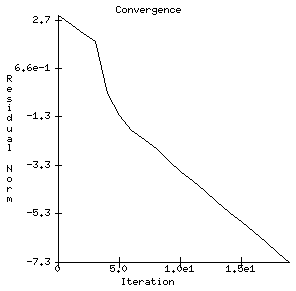
\includegraphics[width=0.9\textwidth]{line-graph-c1tri}
\caption{\PETSc can use X windows to produce line graphs at run time.  (This is not to say they are pretty.)}
\label{fig:line-graph-c1tri}
\end{marginfigure}

Finally, \PETSc can generate graphics showing convergence of iterative methods, at least if X windows are installed.  The line graph in Figure \ref{fig:line-graph-c1tri}, from
\begin{cline}
$ ./c1tri -tri_m 1000000 -ksp_rtol 1.0e-10 -pc_type jacobi \
    -ksp_monitor_lg_residualnorm -draw_pause 1
\end{cline}
%$
shows the residual norm logarithm versus the iteration number.

\bigskip
\section{Exercises}

\renewcommand{\labelenumi}{\arabic{chapter}.\arabic{enumi}\quad}
\begin{enumerate}
\item Program \texttt{c1e.c} does redundant work, and a terrible job of load-balancing, because the computation of the factorial $n!$ on the rank $n$ process requires $n-1$ flops.  Modify the code to balance the load almost perfectly, with exactly one divide operation on each \texttt{rank} $>0$ process, by using blocking send and receive operations (\texttt{MPI\_Send(),MPI\_Recv()}) to pass the result of the last factorial to the next rank.  (\emph{Now the code does lots of communication and waiting.})
% e1balanced.c
\item Show \eqref{introconvergethm}.
\item As the reader will undoubtedly experience, segmentation faults and memory leaks are inevitable when one develops \PETSc codes.  A standard tool for detecting/diagnosing these is \texttt{valgrind}.\sidenote{\href{http://valgrind.org/}{valgrind.org}}  We recommend running it frequently.  As an exercise, run
\begin{cline}
valgrind ./c1vecmatksp
\end{cline}
to see what \texttt{valgrind} shows for a leak-free program.  Then comment-out a \texttt{VecDestroy()} call in \texttt{c1vecmatksp.c} and rerun to see a common type of memory leak.
\item Consider Richardson iteration in the example
\begin{cline}
./c1tri -tri_m 100 -ksp_monitor -ksp_type richardson
\end{cline}
Un-preconditioned Richardson iteration fails (i.e.~add \texttt{-pc\_type none}); explain.  The default preconditioner succeeds (i.e.~\texttt{-pc\_type ilu}), but ILU($0$) is cheating because it becomes a complete LU factorization on this tridiagonal and diagonally-dominant $A$; we are really seeing a direct solve.  The same can be said for ICC($0$).  Confirm that, as in the example on page \pageref{introprerichardson}, Richardson iteration succeeds with \texttt{-pc\_type jacobi}, even though the diagonal is constant; explain.
\item \label{exer:computeeigs} Un-preconditioned GMRES solves the linear system in \texttt{c1tri.c} reasonably efficiently.  We can explain this by asking \PETSc to compute the eigenvalues of $A$ by using option\sidenote{The relevant \PETSc manual page says this option is ``intended only for assistance in understanding the convergence of iterative methods, not for eigenanalysis.  For accurate computation of eigenvalues we recommend using the excellant package SLEPc.''}
\begin{quote}
\texttt{-ksp\_compute\_eigenvalues}
\end{quote}
Because otherwise it computes the eigenvalues of the preconditioned operator $P^{-1}A$, add \texttt{-pc\_type none}.  Try dimensions $N=10,100,1000$.  Why does the  run
\begin{cline}
./c1tri -tri_n 1000 -pc_type none -ksp_compute_eigenvalues
\end{cline}
only show 11 eigenvalues of this $1000\times 1000$ matrix?  How do these eigenvalues explain the good behavior of unpreconditioned GMRES?\sidenote{See \citep{TrefethenBau} for help with both of these questions.}
\item The accuracy of direct solves (e.g.~\texttt{-ksp\_type preonly -pc\_type cholesky}) in \texttt{c1tri.c}, as measured by the reported error norm $\|\bx - \bx_{\text{exact}}\|_2$, decreases with increasing dimension.  Confirm and explain this observation.
\item Table \ref{tab:c1tritiming} includes a number of blanks.  For each one, explain why it is blank, experimenting if needed.
\item Table \ref{tab:c1tritiming} gives execution times not iteration count.  Generate the corresponding table of \pKSP iteration count by adding option \verb|-ksp_converged_reason| to the run commands.  Note the large number of ``coincidences'' in iteration count, i.e.~cases where iteration counts are identical; explain.  Which preconditioners have a strong or weak effect on iteration count?  Is timing or iteration count more useful?
\end{enumerate}